\documentclass{VUMIFPSkursinis}
\usepackage{algorithmicx}
\usepackage{algorithm}
\usepackage{algpseudocode}
\usepackage{amsfonts}
\usepackage{amsmath}
\usepackage{array}
\usepackage{bm}
\usepackage{caption}
\usepackage{color}
\usepackage{float}
\usepackage{graphicx}
\usepackage{listings}
\usepackage{longtable}
\usepackage{subfig}
\usepackage{wrapfig}
\usepackage{enumitem}
\usepackage{pdfpages}

\usepackage[tableposition=top]{caption}
%PAKEISTA, tarpai tarp sąrašo elementų
\setitemize{noitemsep,topsep=0pt,parsep=0pt,partopsep=0pt}
\setenumerate{noitemsep,topsep=0pt,parsep=0pt,partopsep=0pt}

\newcolumntype{L}[1]{>{\raggedright\let\newline\\\arraybackslash\hspace{0pt}}m{#1}}
\newcolumntype{C}[1]{>{\centering\let\newline\\\arraybackslash\hspace{0pt}}m{#1}}
\newcolumntype{R}[1]{>{\raggedleft\let\newline\\\arraybackslash\hspace{0pt}}m{#1}}

% Titulinio aprašas
\university{Vilniaus universitetas}
\faculty{Matematikos ir informatikos fakultetas}
\department{Programų sistemų katedra}
% \papertype{Praktikos ataskaita}
\title{Profesinės praktikos ataskaita}
\status{4 kurso 5 grupės studentė}
\author{Gabrielė Žielytė}
\supervisor{Lekt. Irus Grinis}
\date{Vilnius – \the\year}

% Nustatymai
% \setmainfont{Palemonas-2.1}   % Pakeisti teksto šriftą į Palemonas (turi būti įdiegtas sistemoje)

%--------------------------------------------------------
%----------------------- PRADŽIA ------------------------
%--------------------------------------------------------
\bibliography{bibliografija}
\begin{document}
\maketitle

\setcounter{page}{2}

\tableofcontents

%--------------------------------------------------------
%------------------------ ĮVADAS ------------------------
%--------------------------------------------------------

\sectionnonum{Įvadas}
Profesinė praktika buvo atlikta „Intrum“ grupės bendrovėje „Intrum Global Business Services“. Pasirinkau šią darbovietę, nes norėjau, kad įmonė, kurioje atliksiu praktiką, būtų ne lietuviško kapitalo ir joje galima būtų įgyti ne tik programavimo įgūdžių, bet ir bendradarbiauti anglų kalba. Taip pat buvo tekę girdėti, kad šioje įmonėje yra suteikiamos gana geros darbo sąlygos. Vienintelę darbo patirtį prieš tai turėjau UAB „Asvela“, individualiai kuriant internetinę svetainę šiai įmonei, todėl niekada neturėjau patirties dirbant komandoje, išskyrus grupinius projektus universitete.

Išgirdau, jog šios įmonės testuotojų komanda ieško naujų darbuotojų - tai sudomino, kadangi visuomet norėjau sužinoti, kaip tiksliai atrodo testuotojų darbo diena. Pakalbėjus per darbo interviu, sužinojau, jog šiai komandai labai praverstų programavimą studijuojantis žmogus, galintis parašyti jiems tam tikrą kodą ataskaitų kūrimo automatizavimui, todėl įgaučiau tiek patirties programuojant, tiek rašant testus sudėtingoms įmonės sistemoms bei testuojant. 

Šios praktikos pagrindinis tikslas buvo patobulinti studijose įgytas programavimo, bei testavimo žinias ir šiuos gebėjimus pritaikyti praktikoje, kuriant reikšmingas programas, padėsiančias darbuotojams tolimesnėje įmonės veikloje. Taip pat tikslinga susipažinti su didelių projektų ir sistemų valdymu, bei skirtingas pareigas atliekančių komandų bendradarbiavimu siekiant vieno tikslo.

Praktikos tema buvo „Failų ataskaitos parengimas ir testavimas“. Siekdama įgyvendinti praktikos vadovo prašymus ir tikslus, atlikdama praktiką susidūriau su šiais uždaviniais:
\begin{itemize}
    \item kodo parengimas Python kalba, kuris surinktų informaciją apie failus ir jų būsenas;
    \item failų būsenų ir informacijos juose ataskaitos parengimas web puslapio formatu;
    \item įsigilinimas į naujus sistemos reikalavimus, testų scenarijų ruošimas bei testavimas.
\end{itemize} 

Pirmąją praktikos dieną buvau supažindinta su įmonės biuro aplinka, bendrąja tvarka, keliais bendradarbiais, tiek, kiek galėjo leisti pandemijos paveiktos darbo organizavimo taisyklės. Buvo pristatyta darbo vieta ir suteikti reikiami įrankiai. Šią ir kitą dieną buvo nustatomos ir valdomos reikalingos prieigos teisės, aprodomos pagrindinės sistemos, su kuriomis tenka dirbti testuotojų komandai.

Gavus reikiamas prieigas, vyko pokalbis su komandos vadovu, kuris paaiškino, ko šiuo metu trūksta darbuotojams, bei buvo aptarti jo lūkesčiai ir bendras darbo veiklos planas. Praktikos metu teko labiau įsigilinti į Python kalbos ypatybes, taip pat panaudoti JavaScript, HTML ir CSS kalbų žinias, įgytas universitete. 

Praktikos užduotys susidėjo iš dviejų dalių: programavimo ir testavimo. Programavimo dalyje reikėjo parengti svetainę, atvaizduojančią patogiai parengtą ataskaitą apie į sistemą sukeltus failus su duomenimis apie skolų bylas. Šios užduoties tikslas buvo palengvinti kasdienį testuotojų ir kitų komandų darbą, renkant informaciją apie minėtus failus. Renkant šią informaciją „rankomis“ yra užtrunkama labai daug laiko ir rezultatai gali ne visada būti tikslūs dėl žmogiškojo faktoriaus padarytų klaidų. Tam kad ši užduotis būtų įvykdyta, teko daug analizuoti gaunamus ir siunčiamus kitoms šalims failus, juos grupuoti ir sudarinėti lenteles, atvaizduojančias svarbiausius faktus apie juos.

Antroji praktikos dalis susidėjo iš susipažinimo su įmonėje naudojamomis skolų išieškojimo sistemomis, testų scenarijų šių sistemų funkcionalumams patikrinti rašymo, bei testavimo. Šiek tiek susipažinus su sistemomis, buvo duota užduotis ištestuoti kelis funkcionalumus, o vėliau pamokyta ir testų scenarijų rašymo ir reikiamos informacijos jiems radimo. Kadangi įmonėje testuoja ne tik testavimo komandos nariai, bet ir kitų komandų darbuotojai, scenarijus teko rašyti gana detaliai, kad būtų aišku visiems gavusiems užduotį kažką ištestuoti. Kad tai galėčiau padaryti, reikėjo ir pačiai gerai perprasti sistemą, nebuvo apsieita ir be mokymosi iš bendradarbių jau paruoštų testų tinkama tema.

Programavimo daliai buvo skirta maždaug 7 savaitės, o testavimo -- 3. Tris su puse savaitės buvo rašomas Python kodas failų analizei,  kitas tris su puse savaitės buvo ruošiama WEB aplikacija, leidžianti patogiai peržiūrėti ataskaitas. Testavimui skirtas laikas susidėjo iš savaitės testavimo, o likusios savaitės buvo skirtos naujų testų scenarijų rašymui ir pokalbiams su kitomis komandomis, norint išsiaiškinti naujų funkcionalumų veikimą ir tikėtinus rezultatus.

Visą programavimo projektą nuo pradžios iki galo dariau individualiai, kartais pasitarus su praktikos vadovu. Manau tai leido man geriau suvokti savo atsakomybes ir kūrybiškai pažvelgti į prašymus, taip pat teko pačiai susiplanuoti darbo procesą ir struktūrizuoti kodą taip, kad būtų aišku ir patogu naudoti praktikos vadovui.

Testavimo užduočių vykdymo metu pravertė „Programų sistemų testavimo“ dalyko metu įgautas supratimas apie tai, kaip rašyti testų scenarijus, todėl pradėjus praktiką testų rašymo mokymai neišgąsdino ir galima buvo greitai perimti komandos perleistus darbus. Daugiausiai laiko atliekant testavimo užduotis pareikalavo tai, kad buvo dirbama su visiškai nepažintomis skolų išieškojimo valdymo sistemomis, o tai reiškia, jog reikėjo susipažinti ir su skolų išieškojimo procesu, dalyviais ir rezultatais. 

Užregistravus funkcionalumo klaidą testavimo metu, jos taisyti imdavosi žmonės iš skirtingų komandų, kartais esančių netgi skirtingose šalyse, todėl tikrai buvo patobulintos anglų kalbos žinios, įgauta patirtis dirbant multikultūrinėje įmonėje.

Įdomiausia užduotis, man asmeniškai, buvo pateikti didelį informacijos kiekį WEB aplikacijoje, taip, kad vartotojams būtų intuityvu ir patogu ją naudoti, pernelyg neapkraunant aplikacijos nereikalingomis detalėmis ar prastu svetainės dizainu. Šiai užduočiai labai padėjo universitete įgauti pagrindai apie aplikacijų dizainą, bei WEB aplikacijų kūrimo įrankius (JavaScript, HTML, CSS), bet teko gilintis ir į anksčiau negirdėtas bibliotekas lentelėms ir kalendoriams konstruoti. 


%--------------------------------------------------------
%----------------------- DĖSTYMAS -----------------------
%--------------------------------------------------------

\section {Įmonės apibūdinimas}

„Intrum“ – tai pirmaujanti kreditų valdymo paslaugų teikėja, veikianti 25 šalyse. Bendradarbiaujant su dar su 160 partnerių, ji padeda bendrovėms sėkmingai vykdyti veiklą siūlydama sprendimus, kuriais siekiama užtikrinti sklandesnį pinigų judėjimą, padidinti ilgalaikį bendrovių pelningumą ir rūpintis jų klientais. Labai svarbi „Intrum“ misijos dalis – užtikrinti, kad asmenys ir bendrovės apmokėdami skolas gautų reikiamą pagalbą. Daugiau kaip 10 000 „Intrum“ specialistų teikia paslaugas 80 000 Europos bendrovių. 2020 m. Pajamos siekė 16,85 mlrd. Švedijos kronų. „Intrum“ būstinė yra Stokholme, Švedijoje, o „Intrum“ akcijos kotiruojamos „Nasdaq Stockholm“ biržoje \cite{Intrum}.

„Intrum“ bendrovė Vilniuje buvo įsteigta 2014 m. kaip „Lindorff“ verslo paslaugų centras.„Lindorff“ susijungė su „Intrum Justitia“ ir tapo „Intrum“ – pasaulyje pirmaujančia kredito valdymo paslaugų teikėja. Šiuo metu Lietuvoje veiklą vykdo dvi „Intrum“ grupės bendrovės: kreditų valdymo bendrovė „Intrum Lithuania“ ir „Intrum Global Business Services“ (IGBS). Pastarojoje dirba 400 operacijų specialistų, duomenų analitikų finansų kontrolierių ir kt., kurie atsakingi už „Intrum“ grupės veiklą ir prižiūri verslo tinklą Europos šalyse.\cite{IntrumGBS}

Naudojantis plačiu „Intrum“ kredito valdymo paslaugų spektru, stengiamasi, kad įmonėms būtų sumokėta už jų prekes ar paslaugas.

\subsection{Įmonės misija}
„Intrum“ tikslas yra sukurti bendrą vertę verslui ir visuomenei, pasirūpinant tuo, kad įmonėms būtų mokama laiku, ir piliečiai atsikratytų savo skolų. „Intrum“ nori įnešti ilgalaikį indėlį: ši įmonė bendradarbiauja su verslu, vyriausybėmis ir kitomis suinteresuotosiomis šalimis kuriant patikimą ekonomiką.

Ši įmonė turi biurus 24 Europos šalyse ir vieną Lotynų Amerikoje (Brazilijoje). Turėdami puikų partnerių tinklą, „Intrum“ gali padėti didelėms,  mažoms ir vidutinio dydžio įmonėms ir organizacijoms visame pasaulyje. 

\subsection{Organizacinė struktūra}
„Intrum“ susideda iš daugelio dalių, tačiau šiame darbe bus nagrinėjama tik viena iš jų - „Intrum Global Business Services“ (IGBS), kadangi ten ir buvo atlikta ši praktika. Vilnius buvo pasirinktas „IGBS“ būstine dėl patrauklios išlaikymo ir patalpų kainos, patogios vietos, bei daugybės aukštos kvalifikacijos darbuotojų.

% \vspace{5mm} 
„Intrum Global Business Services“ (IGBS) susideda iš keleto dalių, viena iš jų įsikūrusi Mauricijuje ir yra atsakinga už skambučių centro atliekamas operacija, visos kitos įsikūrusios Vilniuje ir yra atsakingos už įmonės operacijas, verslo analizę, investicijas ir finansus. „IGBS“ dalys (\ref{img:igbs} paveikslėlis):
% \begin{itemize}
%     \item „IGBS Operations“ - operacijų filialas,
%     \item „Operations Center“ - operacijų centras,
%     \item „Accounts Receivable Management & Support“ - sąskaitų valdymas ir palaikymas, 
%     \item „HR & Administration“ - žmogiškieji ištekliai ir administracija,
%     \item „Project Management Office“ - projektų valdymo biuras,
%     \item „Finance and accounting“ - finansų ir apskaitos sektorius,
%     \item „Compliance“ - taisyklių laikymosi užtikrinimo dalis,
%     \item „Intrum GBS Mauritius“ - Mauricijaus skambučių centras.
% \end{itemize}

\begin{figure}[H]
    \centering
    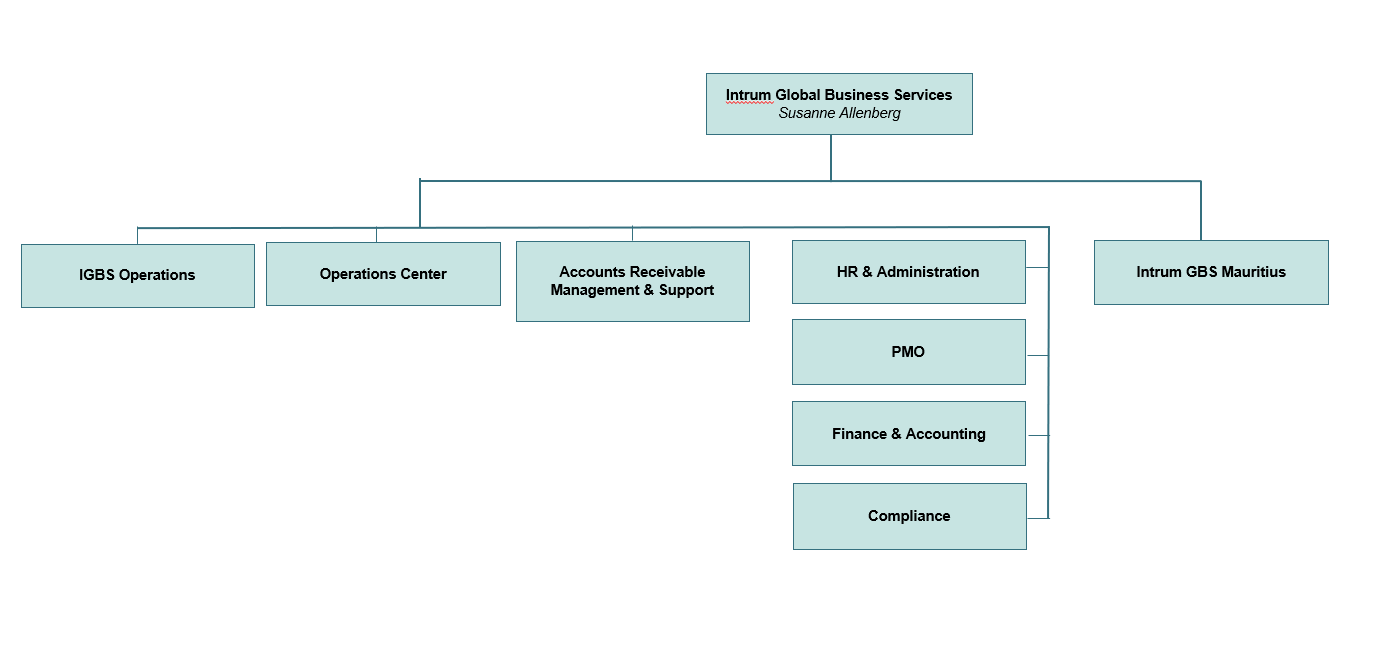
\includegraphics[scale=0.5]{img/IGBS_organizacija.png}
    \caption{„Intrum Global Business Services“ sudėtis}
    \label{img:igbs}
\end{figure}

Praktika buvo atlikta „IGBS“ Operacijų Centre, kuris pats išsiskirsto į dar daugiau dalių: pačių operacijų dalis, jų įgyvendinimo dalis, Operacijų centro verslo partneriai, bei šio centro palaikymo dalis (\ref{img:oc} paveikslėlis)

Operacijų centro įgyvendinimo dalyje yra ir testuotojų komanda, atsakinga už „Intrum“ šalių programinių sistemų bei tinklapių testavimą, testų sudarymą, klaidų radimą ir jų registravimą, stengiantis pagerinti šias sistemas. Kuriant naujus sistemų funkcionalumus, būtina juos ištestuoti, nes vėliau tas sistemas naudos įmonės klientai ir darbuotojai, sprendžiant su skolomis susijusias problemas.

\begin{figure}[H]
    \centering
    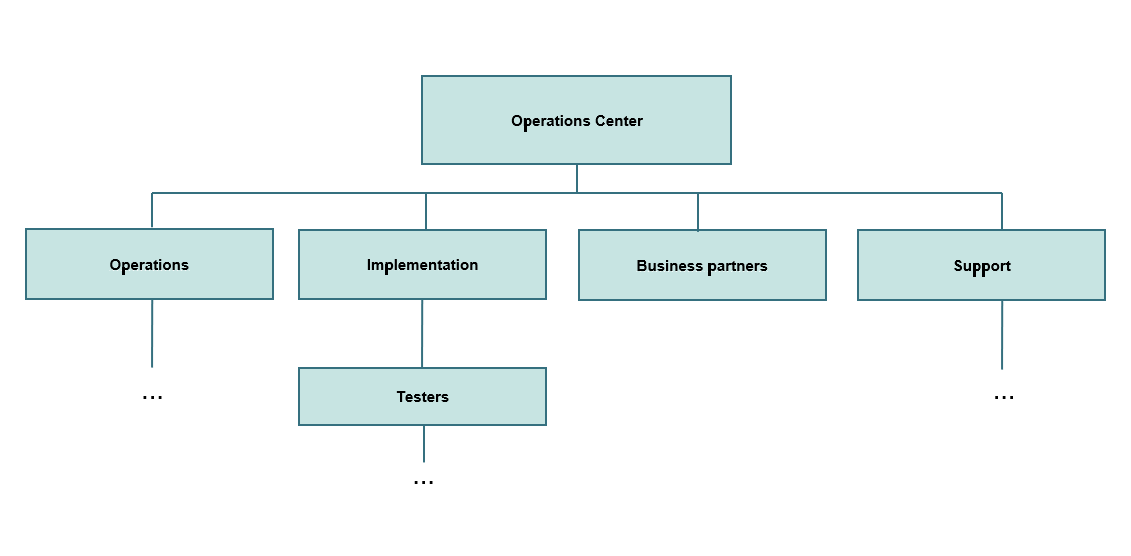
\includegraphics[scale=0.5]{img/OC_sudetis.png}
    \caption{„IGBS Operacijų centro“ sudėtis}
    \label{img:oc}
\end{figure}

\subsection{Darbo sąlygų įvertinimas}

„DUETTO“ verslo centas randasi Spaudos g. 8, Vilniuje. Šiame centre yra 10 aukštų, iš kurių 7 aukštus užima būtent „Intrum“ įmonė, kitus aukštus užima „Vilniaus vandenys“. Tai gana naujas verslo centras, pastatytas 2017 metais. Pirmajame aukšte yra įrengta kavinė, kurioje per pietus paprastai susirenka pastate dirbantys žmonės.

Pirmąją praktikos dieną visiems „IGBS“ naujokams buvo pristatyta įmonė, jos vertybės, struktūra, bei saugos taisyklės. Kiekvienas darbuotojas, priimtas i darbą, gauna magnetinę kortelę, kuria atrakinamos durys į skirtingus aukštus. Darbuotojai gali pasirinkti, nuo kada ryte pradėti darbą: 7-9 val., nuo to priklauso ir laikas, kada galima išeiti namo.

Darbo sąlygos yra labai geros. Visiems darbuotojams suteikiamos atskiros darbo vietos, kompiuteris su dvejais monitoriais, kėdė, ausinės internetiniams susitikimams. Kiekviename aukšte yra virtuvė su nemokama kava ir arbata, visoms atliekoms yra skirtingos šiukšliadėžės rūšiavimui. 

Kadangi praktika buvo atlikta gana sudėtingu laikotarpiu, pandemijos metu, į šią praktikos vietą reikėjo ateiti tik pirmąją savaitę, vėliau kompiuterio dėžutę ir kitus reikiamus įrankius galima buvo pasiimti ir saugiai dirbti iš namų. Naujam darbuotojui visada yra paskiriamas žmogus iš tos pačios komandos, kuris aprodo ofisą, paaiškina nuo ko pradėti, norint paruošti kompiuterį darbui, t.y. kokias programas įdiegti, kaip elgtis su specifinėmis sistemomis, kaip įjungti įmonės „VPN“ ir taip toliau. Būnant darbo vietoje, viską išsiaiškinti yra patogiau, tačiau žinant šiuos techninius dalykus, toliau tęsti darbą buvo įmanoma ir nuotoliniu būdu.

Pirmąją savaitę reikėjo palaukti, kol buvo suteiktos teisės prisijungimams prie sistemų. Visa informacija susijusi su darbu buvo siunčiama įmonės vidiniu elektroniniu paštu, o pokalbiai, bei susirinkimai su bendradarbiais buvo vykdomi „Skype“ arba „Teams“ aplinkose. Pokalbiams buvo naudojamos dvi aplinkos, nes atėjus i praktiką buvo pradėta persikelti iš vienos aplikacijos į kitą.

Praktika buvo atlikta testuotojų komandoje. Jos vadovas kiekvieną rytą rengė susitikimus, kuriuose buvo aptariami kasdieniai darbai ir problemos. Prieš atliekant praktiką, šioje komandoje buvo tik 4 žmonės, tačiau ji pastoviai plėtėsi, ir praktikos pabaigoje komanda buvo išaugusi iki 9 žmonių. Buvo bendradarbiaujama ir su kitų sričių komandomis, vykdomi mokymai. Jei kildavo sunkumų testuojant, visada padėdavo kiti, ilgiau dirbę komandos nariai, o jei kildavo klausimų dėl programavimo dalies buvo kalbama su komandos vadovu, kuris neblogai išmano šią sritį.

Atmosfera komandoje buvo pakankamai maloni, kartais buvo organizuojami žaidimų vakarai, ir tai padėjo naujai prisijungusiems darbuotojams lengviau įsilieti į komandą. Apskritai darbo sąlygos, įskaitant ir darbą nuotoliniu būdu, labai tenkino.


\section{Praktikos veiklos aprašymas}
Pasitarus su praktikos vadovais, buvo apibrėžti tokie praktikos uždaviniai:
\begin{enumerate}
    \item Parengti kodą Python kalba, kuris surinktų informaciją apie failus ir jų būsenas.
    \item Paruošti failų būsenų ir informacijos juose ataskaitą web puslapio formatu.
    \item Įsigilinti į naujus sistemos reikalavimus, paruošti testus ir ištestuoti.
\end{enumerate}

\subsection{Informacijos šaltiniai}
Prieš pradedant, bei įgyvendinant praktikos tikslus reikėjo sukaupti reikiamą žinių bagažą. Informacija buvo renkama naudojantis:
\begin{itemize}
    \item Komandos narių žiniomis ir pagalba. Kuriant ataskaitos ruošimo programą teko konsultuotis su praktikos vadovu, daugiausiai aptariant programos struktūrą ir reikalavimus jai. Testavimo metu teko nemažai klausinėti kitų komandos narių, nes daugelio dalykų negalėjau sužinoti nei dokumentacijoje, nei internete. Labiau patyrę komandos nariai kartais vesdavo mokymus, atsakydavo į dalyviams iškilusius klausimus, duodavo patarimų.
    \item Kitų komandų pagalba. Tekdavo bendrauti ir su įvairiais dalykinės srities specialistais, kurie atsakingi už skolų išieškojimo struktūrą ir operacijas. Pokalbiai su jais leido geriau pažinti šią dalykinę sritį ir sistemos poreikius. Sistemos funkcijos dažnai keičiasi, įvedamos naujos, todėl būtina bendrauti su kitomis įmonės komandomis.
    \item Dokumentacija. Kai kurią informaciją galima buvo rasti arba vidinėje įmonės svetainėje, arba atsiųsdavo kolegos.
    \item Internete esančiomis pamokomis. Ataskaitos ruošimo programa buvo rašoma pagrinde Javascript, HTML, bei Python kalbomis, iš kurių pastarosios nesimokiau universitete, todėl teko pasinaudoti anksčiau savarankiškai įgautomis žiniomis (kuriant kitus projektus), taip pat internete esančiomis pamokomis, programinio kodo pavyzdžiais, bei informacijos apsikeitimo tinklapiais, tokiais kaip „Stack Overflow“ \cite{StackOverflow}.
\end{itemize}

\subsection{Praktikos tikslų įgyvendinimas}

Praktikos uždaviniai susidėjo iš dviejų didelių dalių:
\begin{itemize}
    \item Programavimo dalies - failų būsenų ir informacijos juose ataskaitos ruošimo,
    \item Testavimo dalies - „Intrum“  sistemų testavimo, bei testų rašymo.
\end{itemize}

Pagrindinis testuotojų komandos darbas -- žinoti kokie yra nauji funkcionalumai arba dalykinės srities reikalavimai, parašyti atitinkamus testus ir kai kuriuos iš jų testuoti (kai kuriuos funkcionalumus testuoja kitos „Intrum“ šalys, nes ne visus funkcionalumus galime ištestuoti patys).

\subsubsection{Pirmoji užduotis}
Kartais šios komandos vadovui tenka susidurti su dideliais kiekiais informacijos, bei sudaryti tam tikras ataskaitas, kurios susidarytų greičiau, jei analizei būtų skirtas specialus įrankis. Pirmoji praktikos užduotis buvo susijusi kaip tik su tuo. 

Skirtingoms sistemoms bendraujant tarpusavyje yra siunčiami failai su informacija: 
\begin{itemize}
    \item Ar failai su informacija apie bylas, buvo sėkmingai importuoti į sistemą
    \item Jei nebuvo sėkmingai importuoti, kuriuose failuose ir kuriose eilutėse buvo aptikta klaidų
    \item Kurie failai buvo praleisti
\end{itemize}

Problema buvo tame, kad visą šią informaciją komandos vadovui reikdavo peržiūrėti pačiam, atidarant visus kiekvienos Graikijos skolų išieškojimo agentūros („DCA“) failus. Su vadovu buvo aptarta, jog būtų žymiai patogiau surinkti reikiamą informaciją, jeigu tam būtų skirtas specialus įrankis, geriausia svetainės pavidalu.

Šio projekto įgyvendinimui reikėjo išmanyti ir panaudoti šias kalbas:
\begin{itemize}
    \item Python
    \item HTML
    \item CSS
    \item Javascript
\end{itemize} 
Taip pat reikėjo jas panaudoti norint išanalizuoti „docx“, „csv“ bei „JSON“ failus. Iš esmės, praktikos vadovas tik pasakydavo nuo ko būtų patogiausia pradėti rašyti kodą, o tai, kaip tai padaryti spręsdavau pati.

\subsubsubsection{„Python“ programavimo dalis}
Jau pirmąją savaitę, gavusi reikiamas teises, pradėjau rašyti kodą. Pirmoji užduotis buvo parašyti programą Python kalba, kuri atsiųstų minėtus failus ir aplankus iš įmonės serverio į lokalią kompiuterio atmintį. Tuomet galima buvo pradėti pagrindinę duomenų analizės programos dalį, taip pat rašomą Python kalba. 

Atsisiuntus gautus agentūrų failus, galima buvo sukurti klases skirtingiems failų tipams (tipą galima nuspręsti iš failo pavadinimo pradžios), kurie pasižymi skirtingomis savybėmis:
\begin{itemize}
    \item „IMP“ failas - „imported“ arba gautas failas, kuriame yra saugoma informacija apie tam tikras bylas,
    \item „EXP“ failas - „exported“ išsiųstas failas,
    \item „DCA“ failas, kuriame nurodoma, kurioje failų eilutėje buvo padaryta klaida,
    \item „SKIP“ failas, parodantis kurie failai buvo praleisti.
\end{itemize}
% kuri nuskaitytų esamus failus ir jų būsenas 
Nuskaičius failus, suskirsčius juos pagal tipus ir priskyrus jiems reikiamus, vėliau praversiančius atributus, tokius kaip: data, failo kelias sistemoje, agentūros pavadinimas ir kitus - teko sukti ciklą per visus „DCA“ ir „SKIP“ failus, bei priskirti esamiems „IMP“ ir „EXP“ failams užfiksuotų klaidų sąrašą. Deja „DCA“ failai taip pat turėjo dvi rūšis, todėl reikėjo pritaikyti kodą visiems atvejams. Visi failai buvo „csv“ tipo, reikšmės atskirtos ženklu „|“, todėl nemažai kartų teko pasinaudoti patogia Python funkcija „split“, leidžiančia išskirstyti tekstą pagal nurodytą atskyrimo ženklą. Ši dalis buvo įvykdyta per maždaug pusantros savaitės.

Daugiausiai problemų kilo vėlesniame etape, kuomet, pakalbėjus su praktikos vadovu, buvo tiksliau paaiškinta, kokios informacijos reiktų galutinėje ataskaitoje. Prašymas buvo saugoti informaciją apie tai, kurios tiksliai eilutės buvo importuotos, todėl teko susieti eilutes originaliuose („IMP“, „EXP“) failuose su eilutėmis klaidų failuose („SKIP“, „DCA“) ir pašalinti iš sąrašo tas, kuriose buvo įvykusios klaidos, taip pat pašalinti visas eilutes, jei buvo klaida ne su atskiromis eilutėmis, o visu failu - galbūt neatitiko pavadinimas arba antraštės failo viduje.

Problema iškilo tuomet, kai pastebėjau, jog kartais eilutė klaidų failuose šiek tiek skiriasi nuo originalaus failo - kartais nėra vienos ar kitos reikšmės, bet yra aišku, jog minima ta pati eilutė. Deja parašytas programinis kodas lygino eilutes pagal tai, ar sutampa kiekvienas jų simbolis, todėl buvo aišku, jog reikės tai pakeisti. Šis neatitikimas buvo nepastebėtas netgi praktikos vadovo, todėl teko įrodyti, kad failų eilutės tikrai kartais skiriasi. Šiai problemai spręsti buvo pasinaudota „difflib“ biblioteka, kuri pateikia funkciją, leidžiančią nustatyti panašias reikšmes iš sąrašų tam tikru tikslumu. Tikslumas buvo nustatytas bandymų būdu, buvo lyginamos panašios reikšmės ir žiūrima, kokiu tikslumu jos sutampa. Buvo parinkta optimaliausia tikslumo vertė, kuri veikia visiems atvejams.

Taip pat aptarus šią problemą su vadovu, jis patvirtino, jog kai kurių stulpelių reikšmes, jei jos nesutampa, galima tiesiog ignoruoti. Detaliau panagrinėjus turimą informaciją, pastebėjau, jog dažnai skiriasi ir skaičių formatas, kai kur rašomas tam tikras skaičius nulių trupmeninėje dalyje, kai kur jų nėra.

Pagal šiuos atradimus buvo parašytas programinis kodas, generuojantis „JSON“ tipo failus, suskirstytus pagal datą ir kuriuose kiekvienas importuotas/eksportuotas failas turėjo šias vertes:
\begin{itemize}
    \item sąrašą, kuriame paminėta klaidos žinutė, bylos eilutė, kurioje įvyko klaida originaliame faile, bei eilutė paminėta klaidų faile. Toks sąrašas padėjo nuosekliau atvaizduoti informaciją vėlesniuose užduoties etapuose;
    \item visų tame faile esančių eilučių sąrašą;
    \item visų sėkmingai importuotų eilučių sąrašą;
    \item antraščių pavadinimus;
    \item klaidingų eilučių sąrašą;
    \item eilučių su perspėjimais (angl. \emph{„warning“}) sąrašą. Jis buvo reikalingas dėl to, kad, jei eilutei yra skirtas tik perspėjimas (be rimtos klaidos), ši eilutė yra importuojama į galutinę sistemą, kai klaidingos eilutės nėra importuojamos. \newline
\end{itemize}

Šiam Python kalbos programiniam kodui parašyti reikėjo maždaug trijų su puse savaitės. Ne karta buvo susidurta su netikėtumais, bet pabaigoje jie visi buvo įveikti ir kodas veikė taip, kaip ir turėtų.

\subsubsubsection{Web programavimo dalis}

Turint sugeneruotus duomenis, galima buvo pradėti kurti svetainę, leidžiančią patogiai peržiūrėti šią informaciją su galimybe ją filtruoti ir rūšiuoti. Vadovas turėjo prašymą sukurti svetainę, nereikalaujančią serverinės dalies, tai yra, tokią, kurios HTML puslapį galima būtų peržiūrėti tiesiog naršyklėje. Toks prašymas kilo dėl to, kad šiai įmonei yra labai svarbus saugumas, todėl įmonės kompiuteriuose galima naudoti tik prieš tai patvirtintas programas. 

Prieš pradedant rašyti kodą svetainei, praktikos vadovas atsiuntė svetainės dizaino eskizą su komentarais, parodantį, kokių funkcionalumų reiktų (\ref{img:eskizas} paveikslėlis).

\begin{figure}[H]
    \centering
    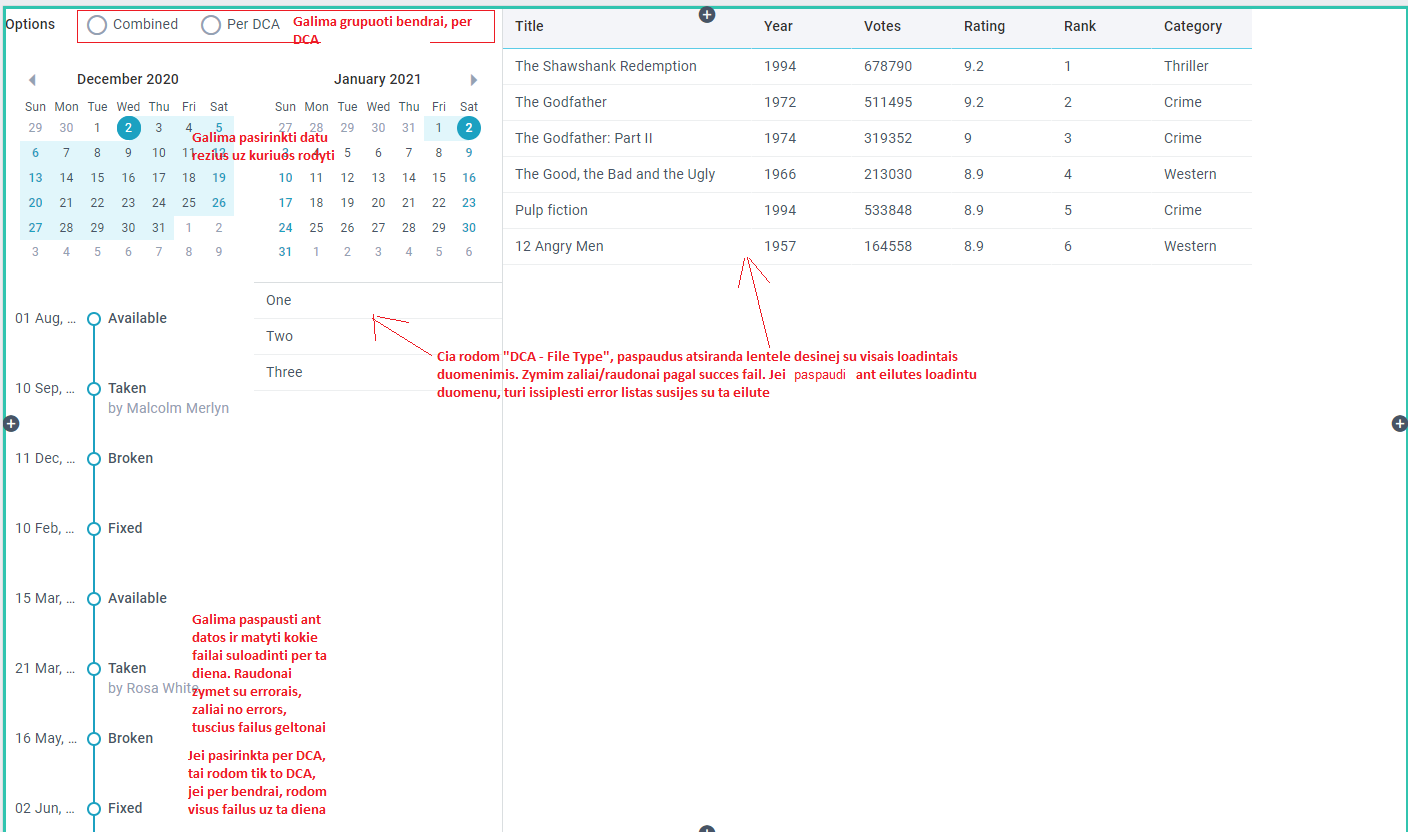
\includegraphics[scale=0.5]{img/eskizas.PNG}
    \caption{Pradinis svetainės eskizas}
    \label{img:eskizas}
\end{figure}

Pasirinkau svetainę kurti pasitelkiant JavaScript bibliotekas:
\begin{itemize}
    \item „Date Range Picker“ datos rėžių pasirinkimui \cite{daterangepicker};
    \item „Tabulator“ interaktyvių lentelių kūrimui \cite{Tabulator}.
\end{itemize}

JavaScript saugumo sumetimais neleidžia pasiekti failų sistemos ir ja manipuliuoti, bet leidžia pasiekti objektus „JSON“ failuose. Dėl šios priežasties reikėjo šiek tiek pakeisti tai, kaip generuojami „JSON“ failai, bei paruošti papildomą failą, kuriame būtų laikomi anksčiau minėtų „JSON“ failų pavadinimai sąrašo pavidalu. Pasinaudojus išvardintomis priemonėmis, buvo galima pridėti reikiamų failų šaltinius į pagrindinį HTML failą. To prireikė, nes kiekvieną dieną daugėja analizei skirtų failų, todėl jų negalima įterpti statiškai.

Per savaitę svetainėje buvo sukurtos keturios lentelės, su rikiavimo ir filtravimo funkcijomis specialiai pritaikytomis užduoties reikalavimams:
\begin{enumerate}
    \item Pirmoji, parodanti sąrašą visų importuotų/eksportuotų failų pasirinktame laiko tarpe, šių failų eilučių (bylų) kiekį, laukus, nusakančius, ar failas buvo sėkmingai įkeltas į sistemą, ar buvo klaidų, arba perspėjimų.
    \item Antroji lentelė pasirodo pirmojoje paspaudus ant kokio nors failo. Joje atvaizduojamos visos to failo eilutės ir šios yra nuspalvinamos raudonai - jei buvo klaidų, žaliai - jei nebuvo, geltonai - jei buvo tik perspėjimų.
    \item Trečioji lentelė pasirodo antrojoje paspaudus ant eilutės, pažymėtos raudonai. Lentelėje nurodomos tikslios klaidų žinutės.
    \item Ketvirtoji lentelė buvo skirta išimtiniams atvejams, kai ne atskiros failų eilutės yra klaidingos, o visas failas. Ši lentelė buvo sukurta tam, kad klaidų žinutės nebūtų kartojamos kiekvienos eilutės lentelėje, atrodytų sistematiškiau.
\end{enumerate}

Vėliau buvo nuspręsta, jog svetainė atrodo per daug apkrauta ir galima sumažinti lentelių skaičių - palikti tris. Vietoj antrosios ir trečiosios lentelių buvo sukurta lentelė, išvardijanti visas failo eilutes, ir kiekviena jų yra nuspalvinama atitinkamomis spalvomis, pagal tai, ar joje įvyko klaida.

Svetainei įgaunant galutinį pavidalą, buvo paprašyta įterpti dar kelias funkcijas:
\begin{itemize}
    \item galimybę nerodyti lentelėse tuščių failų,
    \item galimybę atsisiųsti lentelę HTML formatu,
    \item galimybę sugeneruoti tam tikrų failų statistiką, bei ją atsisiųsti,
    \item galimybę šalia klaidų žinučių matyti jų paaiškinimus, kurie būtų gaunami iš įmonės sukurto specifikacijos dokumento.
\end{itemize}

Paskutiniajam prašymui įgyvendinti, reikėjo parašyti Python kalbos programinį kodą, kuris pasiektų klaidų žinučių aprašymus tam skirtame dokumente ir sugeneruotų „JSON“ failą su reikiamais paaiškinimais. Šio failo informacijos pagalba, į svetainės paskutinę lentelę galima buvo įtraukti ir papildomą eilutę-lentelę su paaiškinimais kada įvyksta tam tikra klaida.

Per maždaug tris savaites buvo sukurta svetainė įgyvendinanti visus reikalavimus (\ref{img:svetaine} paveikslėlis). Per šį laiką ne kartą buvo keičiamas dizainas, kad būtų patogiau naudoti vartotojams. 

% Kiekvieną kartą paleidus svetainę yra pakraunami visi duomenų failai, matomas pakrovimo langas. Viską pakrovus pasirodo puslapis, susidedantis iš kalendoriaus, kuriame pasirenkami datos rėžiai, bei dvi lentelės

\begin{figure}[H]
    \centering
    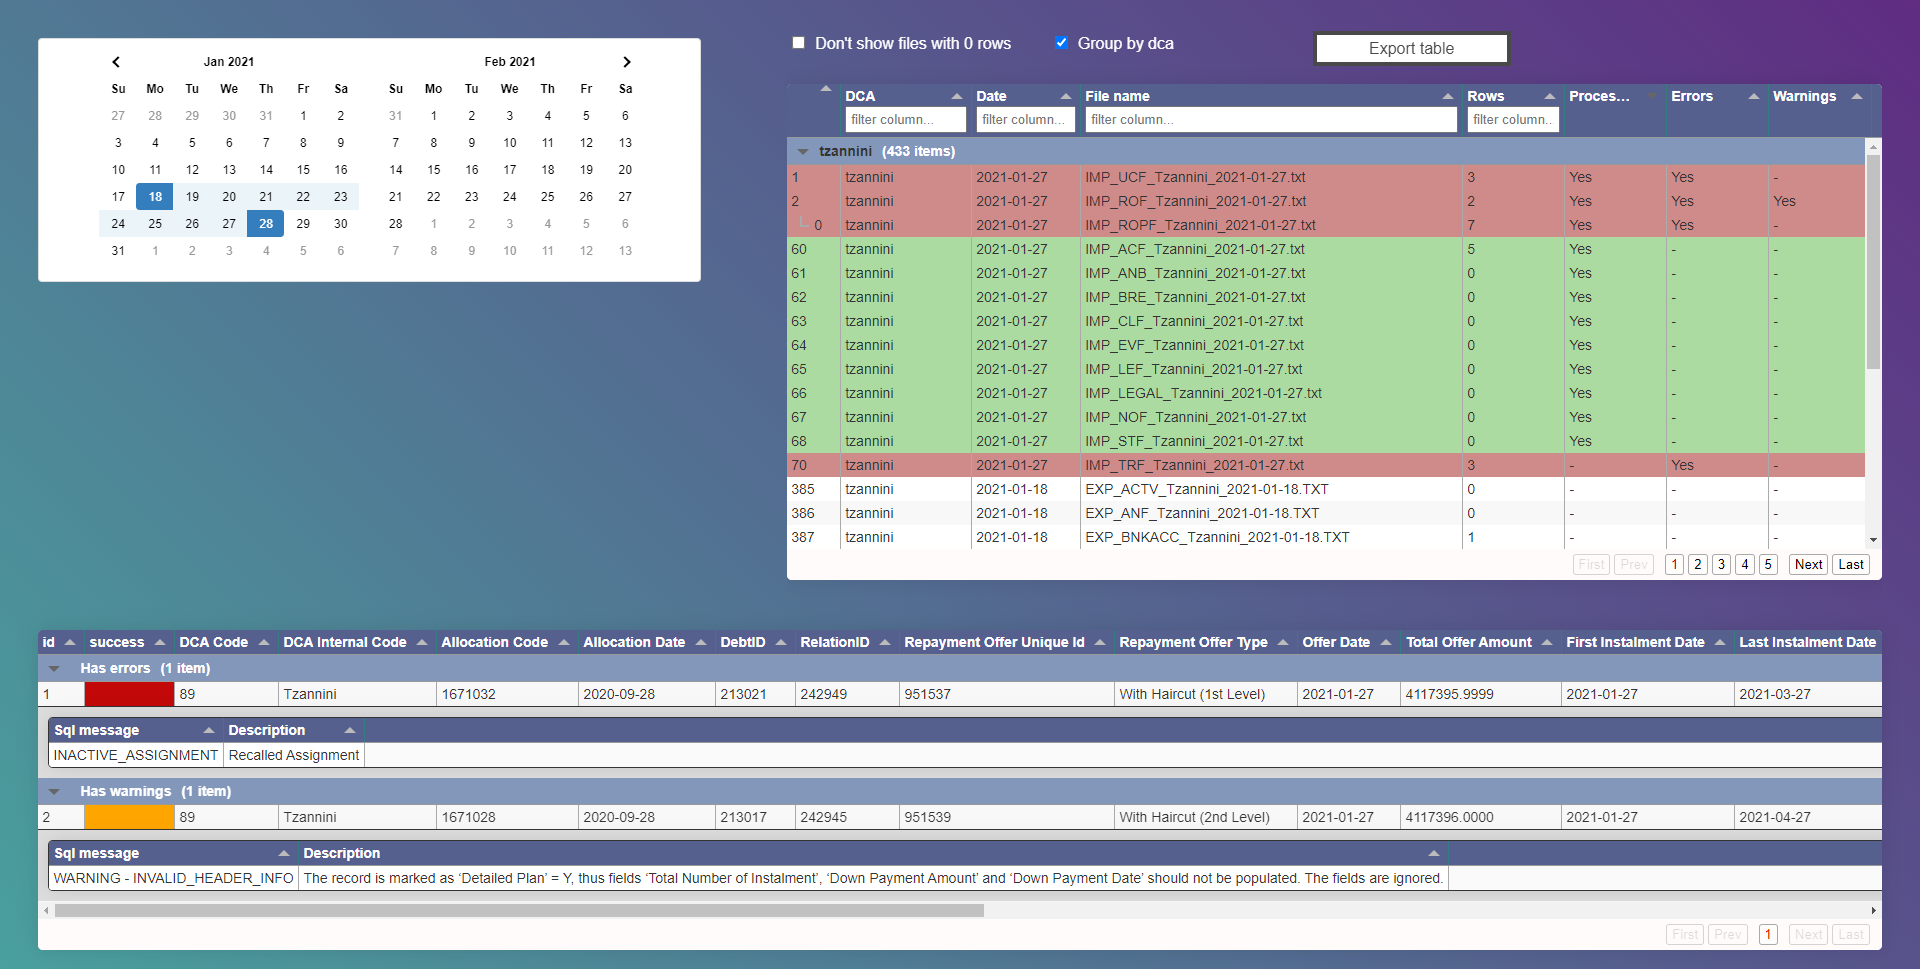
\includegraphics[scale=0.35]{img/svetainesVaizdas.png}
    \caption{Galutinis svetainės vaizdas}
    \label{img:svetaine}
\end{figure}
\newpage
\subsubsection{Antroji užduotis}

Po programavimo dalies buvo metas susipažinti su įmonėje dirbančių testuotojų kasdieniais darbais. Jie susidėjo iš nuolatinio bendravimo su kitomis komandomis, norint išsiaiškinti tinkamą sistemos veikimą, testuojamų sistemų funkcionalumų mokymosi, testų scenarijų rašymo bei testavimo ir, žinoma, klaidų registravimo. Šiems testuotojams reikia nuolatos mokytis, nes testuojamų sistemų funkcionalumų kiekiai yra labai dideli, be to kai kurie skiriasi priklausomai nuo šalies. 

Testavimo komanda dirba su įmonės skolininkų bei klientų pusės svetainių funkcionalumus, bei visų „Intrum“ šalių „Qualco“ sistemas, valdančias su skolų išieškojimu susijusius veiksmus. „Qualco“ -- tai skolų portfelių valdymo sistemų ir technologijomis pagrįstų paslaugų teikėjas, apimantis visus skolų išieškojimo gyvavimo ciklo aspektus.

Pirmoji man skirta testavimo užduotis buvo ištestuoti maždaug 15 Danijos „Qualco“ sistemos funkcionalumų. Gavus užduotį man paskyrė ir komandos narį, kuris parodytų kaip veikia sistema, kaip įkelti bylas į šią sistemą, bei kaip rašomi testai. Kiti komandos nariai taip pat pravedė kelias paskaitas apie „Jira“ sistemą, kuri yra patentuotas „Atlassian“ sukurtas problemų stebėjimo produktas, leidžiantis sekti klaidas ir užtikrinti judrų projektų valdymą. Šios paskaitos padėjo bent minimaliai perprasti naudojamus įrankius. Nepaisant to, pradėjus daryti pirmąjį testą, iškart kilo nesklandumų, todėl turėjau klausti bendradarbių, ką tokiu atveju daryti.

Testuojant šiuos Danijos sistemos funkcionalumus, ne kartą iškilo neaiškumų, bet visuomet padėdavo kiti komandos nariai. Buvo užregistruota nemažai sistemos klaidų, aprašyta, ką darant šios klaidos kilo, bei jos visos buvo ištaisytos kitų „Intrum“ darbuotojų pagalba. Buvo tikėtasi, jog šis scenarijus bus ištestuotas per savaitę, bet realybėje šis laikotarpis prasitęsė iki maždaug dviejų, dėl didelio klaidų funkcionalumuose skaičiaus, bei to, kad teko laukti ne vieno „End of Day“ -- laikotarpio dienos pabaigoje, per kurį įkeliami ir atnaujinami duomenys -- o klaidų radimo atveju, reikėjo ne kartą ištestuoti tą patį funkcionalumą, atsiradus pataisymams. 

Kadangi testuojant tekdavo laukti „End of Day“-- kol bus importuoti duomenys, laukimo metu komandos nariai pamokė, kaip reiktų kurti pačius testus. Kiekvienas iš testuotojų koncentruojasi į skirtingas sistemų vietas, man paskyrė dirbti su „Action Networks“ sritimi, kur testų scenarijai yra rašomi pagal brėžinius, parodančius per kokius etapus keliauja įkelta skolos byla (\ref{img:brezinys} paveikslėlis). Pradžiai rašiau testus „mažoms“ strategijoms, tokioms, kokia yra \ref{img:brezinys} paveikslėlyje, vėliau perpratus specifinius žymėjimus ir brėžiniuose žymimus laiko matavimus, galima buvo pereiti prie didesnių schemų, susidedančių iš daugelio atšakų ir, kurių testavimas tęsiasi galbūt netgi kelias savaites. Praėjus vieną strategiją skolos byla gali nueiti į kitą, taip keliaudama iki pat jos uždarymo pabaigos.

\begin{figure}[H]
    \centering
    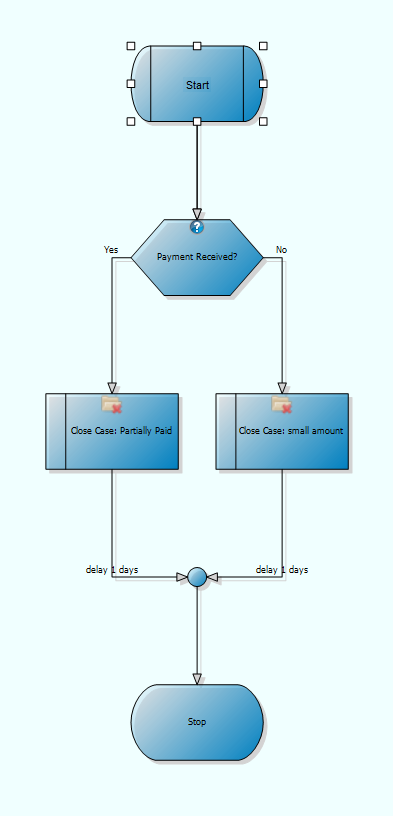
\includegraphics[scale=0.5]{img/smallAmountsver2.png}
    \caption{Bylos kelionės brėžinys}
    \label{img:brezinys}
\end{figure}

Kartais yra parašomi testų scenarijai, bet dar nespėjus jų ištestuoti, sistemos arba atskirų funkcionalumų versija pasikeičia, todėl reikia keisti ir scenarijus. Pateiktame didesnės schemos pavyzdyje (1 priedas) matoma, jog bylos kelias yra apibrauktas, tam, kad testuotojams arba tiems, kurie vėliau turės pakeisti scenarijų, būtų aiškiau, kokiu keliu byla keliavo. Šioje schemoje taip pat yra matomi skirtingi žymėjimai, kurių reikšmę koreguoja „Action Networks“ komandos nariai, todėl be jų pagalbos nebuvo apsieita. 

Minėtai schemai buvo parašytas testavimo scenarijus (2 priedas), susidedantis iš 17 žingsnių ir kurį testuoti truktų maždaug 8 dienas (jei neiškiltų nesklandumų). Tokie scenarijai yra registruojami svetainėje „Jira“, ir testuotojai kiekvieną žingsnį gali žymėti kaip sėkmingą, nesėkmingą, arba vykdomą. Taip pat prie kiekvieno žingsnio galima pridėti pastabų arba prisegti iškilusį defektą. Visi testai yra rašomi anglų kalba.

Kartais daugiau informacijos apie tai, ką reiškia schemos objektas, arba tai, koks veiksmas turi būti priskirtas bylai, galima pamatyti šalia schemos esančioje lentelėje, kuri pasirodo paspaudus ant minimo objekto.

Daugiausiai problemų iškildavo dėl tokių žingsnių kaip „laiško nusiuntimas klientui“, nes laiškų šablonai skiriasi kiekvienai šaliai ir komanda atsakinga už šiuos laiškus kartais nespėja jų įkelti į sistemą. Taigi netgi įvykdžius laiško siuntimo žingsnį jis sistemoje nesusigeneruoja taip, kaip turėtų būti pagal testavimo scenarijų. Reiktų paminėti, jog testuojamos „Qualco“ sistemos yra trijų aplinkų (angl. \emph{„environment“}): 
\begin{itemize}
    \item „TEST“ -- skirta testavimui ir bandymams;
    \item „UAT“ -- skirta testavimui specifinės šalies viduje;
    \item „PROD“ -- naudojama realių darbuotojų.
\end{itemize}
Jei testus vykdo Operacijų Centro darbuotojai, naudojama „TEST“ aplinka, jei juos vykdo tam tikros šalies darbuotojai (ne testuotojai), naudojama „UAT“ aplinka.

Šiuo metu yra rašomi gana detalūs scenarijai, yra patikslinama, kuriuos laukus testuotojui reikia patikrinti, kartais parašoma kaip tiksliai rasti kelią programoje, norint pasiekti funkcionalumą. Taip daroma dėl to, kad testuoja ir nedaug su sistema susipažinę darbuotojai.

Per keletą savaičių labiau pažinau įmonės testuojamas sistemas, taip pat išmokau rašyti testus, nors dažnai vis tiek tekdavo pasikonsultuoti su bendradarbiais dėl kai kurių detalių, kurios būdavo neaiškios. Parašiau maždaug 13 skirtingų testų scenarijų, ir prieš kiekvieną iš jų atiduodant testuoti parodydavau atliktus darbus kolegai, kad nepalikčiau klaidų dėl savo patirties dirbant su šiomis sistemomis trūkumo.

\section{Apibendrinimas}

\subsection{Rezultatai ir išvada}

Galiu išskirti praktikos metu pasiektus rezultatus:
\begin{itemize}
    \item pasiekti visi praktikos metu išsikelti uždaviniai;
    \item parašyta apie 530 Python ir 680 JavaScript programinio kodo eilučių;
    \item ištestuota 15 funkcionalumų;
    \item parengta 13 testų;
    \item praktikos metu sukurta svetainė naudojama įmonės kasdienėje veikloje.
\end{itemize}
\bigskip

Sukurta ataskaitos generavimo sistema ženkliai palengvino kasdienį kelių testuotojų darbą, kadangi jiems nebereikia „rankomis“ rinkti informacijos atskirai atidarant failus -- už juos tai padaro parašyta sistema, ir informacija patogiai pateikiama svetainėje arba atsisiuntus iš jos statistikos ataskaitą.

Buvo įgauta daugiau patirties su tokiomis programavimo kalbomis kaip Python serverinei daliai ir JavaScript klientinei daliai. Taip pat susipažinta su „Jira“ įrankiu, bei sudėtingomis įmonės sistemomis, paremtomis „Qualco“, buvo sėkmingai taikyti „Agile“ principai, nes kiekvieną dieną buvo rengiami komandos susirinkimai atliktiems arba būsimiems darbams atlikti. 

Buvo panaudotos universitete įgytos žinios apie skirtingus algoritmus, svetainių kūrimą, bei bendrą testų rašymo praktiką. Šios žinios ir universitete įgautas požiūris į atliekamą veiklą bei savarankišką mokymąsi labai padėjo praktikos metu neišsigąsti sunkumų atliekant paskirtas užduotis. 

Nors praktika buvo atliekama pandemijos laikotarpiu, tai nesutrukdė sklandžiam darbų pasiskirstymui, mokymams ir pačiam darbui. Viską galima buvo aptarti „Teams“ susirinkimų metu, esant savo namuose, o susipažinimas su bendradarbiais vyko virtualių susitikimų metu, žaidžiant žaidimus.

\subsection{Praktikos trūkumai ir privalumai}

Praktikos metu atliekant įvairias užduotis, buvo įgyta daug naudingos patirties, bei sužinoti ir panaudoti nauji įrankiai, sklandžiam darbui vykdyti. Taip pat buvo suteikta galimybė susipažinti su dideliu kiekiu naujų žmonių, ne vien iš Lietuvos, praplėsti savo akiratį, patobulinti anglų kalbos žinias. Kadangi praktika buvo atlikta didelėje kompanijoje, buvo pamatyta kaip atliekami skirtingi darbai, kaip pildomi prašymai prieigai prie reikalingų sistemų, kaip yra užtikrinamas aukšto lygio saugumas, bei kaip skirtingų sričių komandos bendradarbiauja tarpusavyje.

Pagrindiniai praktikos trūkumai tai komandinio darbo trūkumas atliekant programavimo užduotis, bei informacijos trūkumas naujai atėjusiems darbuotojams. Nors ir buvo vykdomi mokymai, apie tai, kaip veikia sistemos, informacijos yra per daug vien išsakymui jos per susitikimus - būtų gerai, jei būtų paruošta dokumentacija su instrukcijomis, nes naujai priimtiems darbuotojams reikia nemažai laiko vien susipažinimui su sistema, gilesniam supratimui įgauti laiko reikia dar daugiau. 

Tai, jog programavimo užduotis visuomet atlikdavau viena yra ir privalumas ir trūkumas, nes iš dalies įgavau nemažai patirties pati priimdama sprendimus, bet iš kitos pusės būtų buvę naudinga bendradarbiauti su kitais ir mokytis vieniems iš kitų, nes atlikus kokį nors sprendimą ne visada žinodavau, ar jis tikrai yra tinkamas.

\subsection{Pasiūlymai}
Praktikos metu buvo įžvelgti keli trūkumai susiję su naujų darbuotojų mokymu apie esamas sistemas. Mano praktikos laikotarpiui įpusėjus į testuotojų komandą atėjo bent 4 nauji žmonės, ir nors kartais vyko mokymai, buvo galima matyti, jog visiems yra sunku apsiprasti su esamomis sistemomis, nes jos turi begalę funkcionalumų. Mano pasiūlymas būtų komandos vadovui ar ilgiau komandoje dirbusiems žmonėms sudaryti mokymų planą, galbūt paruošti video paskaitas ar dokumentaciją, kad nereiktų kaskart atėjus naujiems žmonėms pasakoti to paties, daugiau laiko skirti gilinimuisi į šias sistemas. 

Turėčiau kelias pastabas universiteto darbo organizavimui praktikos metu - pagrinde, tai pajutau organizuotumo trūkumą renkant parašus ir pildant galutines įvertinimo anketas. Pandemijos laikotarpis tikrai paveikė universiteto veiklą, todėl negalima kieno nors per daug kaltinti, tačiau nuotolinė praktika buvo vykdoma jau antrą kartą, todėl buvo keista, kad informacija, apie tai kokie yra įmanomi būdai surinkti dėstytojo ir praktikos vadovo parašus, buvo pateikta tik kelioms dienoms prieš sutarčių pasirašymo galutinę galimą datą. Jautėsi sumišimas tarp studentų, kadangi nebuvo aišku, ar bus galima pasirašyti elektroniniu būdu, kai kurie neturėjo prieigos prie skenerių ar spausdintuvų, nes netgi spausdinimui skirtos viešos vietos buvo uždarytos. Tuo metu daugelis studentų rašė laiškus studijų skyriui apie tas pačias problemas, todėl kitu nuotolinių praktikų metu siūlyčiau suteikti daugiau informacijos studentams, kad studijų skyriaus darbuotojai nebūtų taip apkrauti laiškais ir patiems studentams būtų aiškiau.

\printbibliography[heading=bibintoc]

\appendix
\section{Skolos bylos kelionės diagrama}
Pavyzdys didesnės bylos kelionės diagramos dalies, kuriai buvo rašomas testavimo scenarijus. Šiai diagramai rašytas scenarijus yra antrajame priede.

\begin{figure}[H]
    \centering
    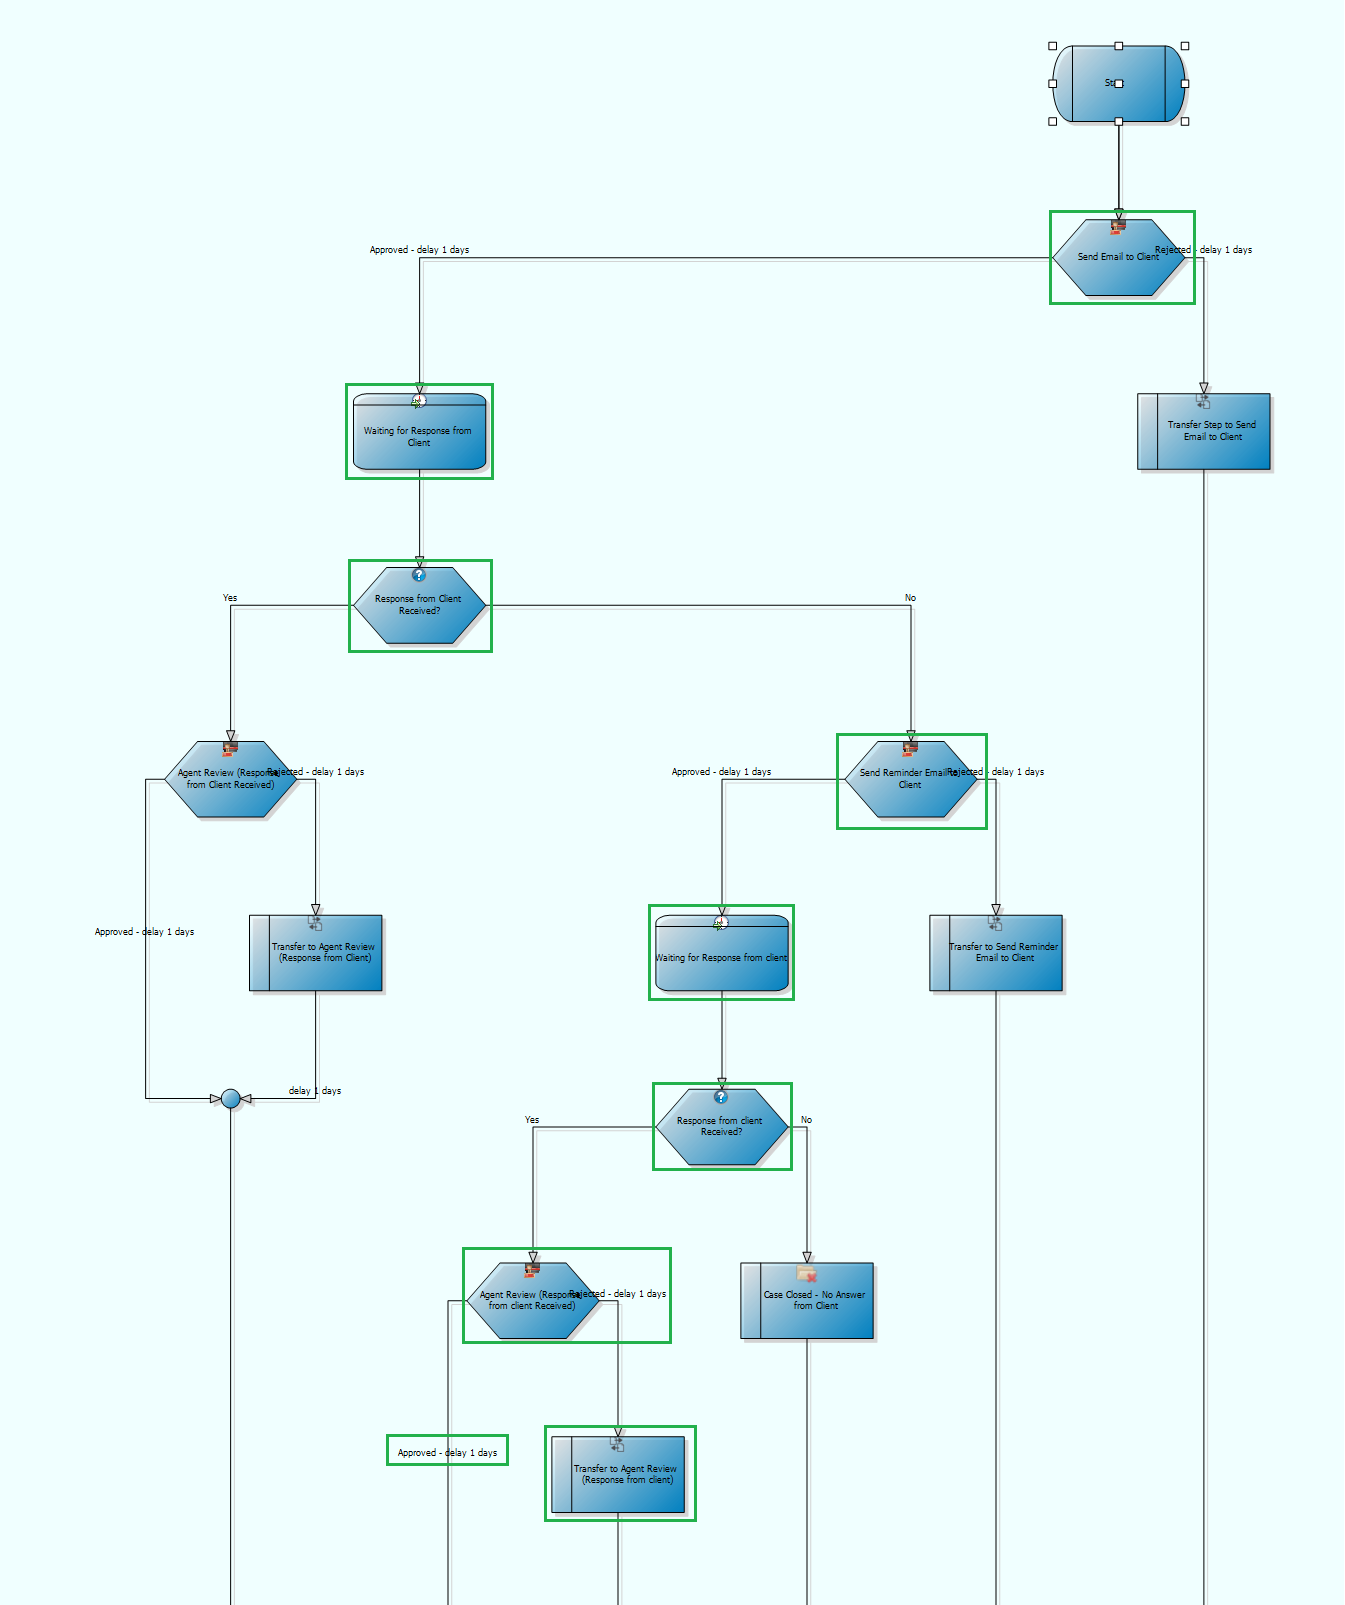
\includegraphics[scale=0.4]{img/Pending legal decision2.png}
    \caption{Didesnis bylos kelionės brėžinys}
    \label{img:brezinysDid}
\end{figure}

\section{Testavimo scenarijus}
Pavyzdys pirmajame priede matomos bylos kelionės dalies testavimo scenarijus.

\begin{figure}[H]
    \centering
    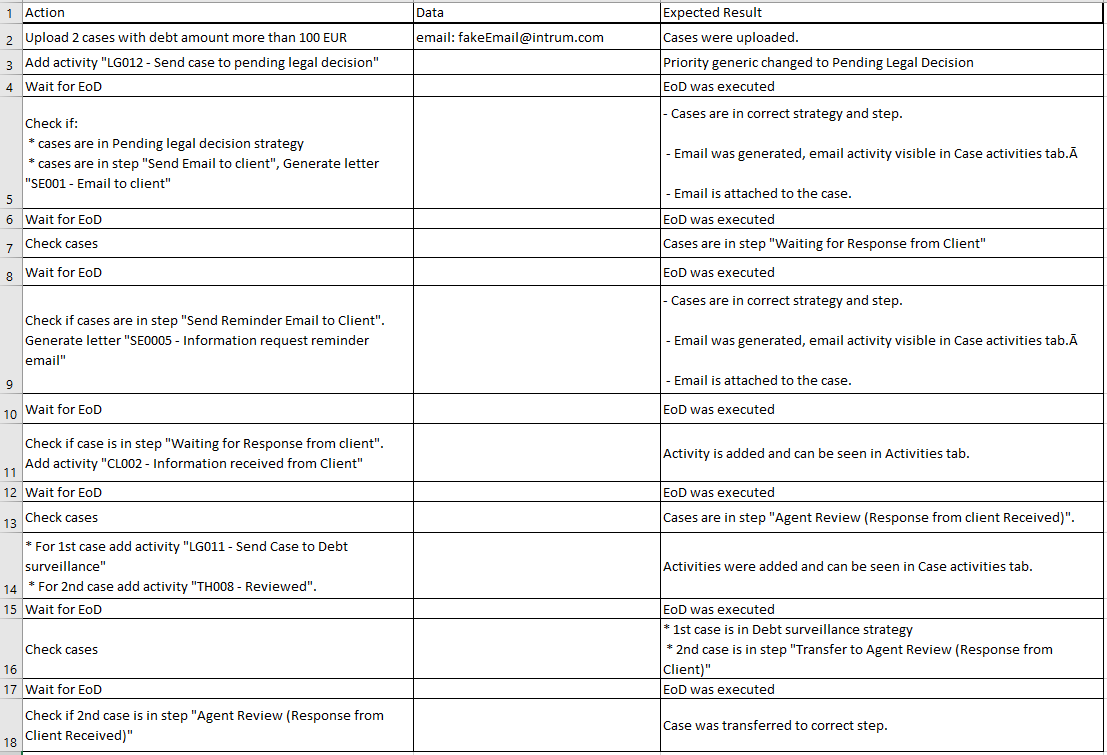
\includegraphics[scale=0.6]{img/testCaseExcel.png}
    \caption{Testavimo scenarijus}
    \label{img:testScenarijus}
\end{figure}

%--------------------------------------------------------
%----------------------- PRIEDAI ------------------------ 
%--------------------------------------------------------

\end{document}